\section{Results}
\label{sec:swave:meas:res}

The results of the fit to each of the \qsq bins for the \Bd mass spectrum are shown in Fig.~\ref{fig:swave:meas:fits:1} and for the \kpi mass spectrum are shown in Fig.~\ref{fig:swave:meas:fits:2}.
\begin{figure}[tbp]
\centering
\subfigure[$0.10<\qsq<2.00\gevgevcccc$]{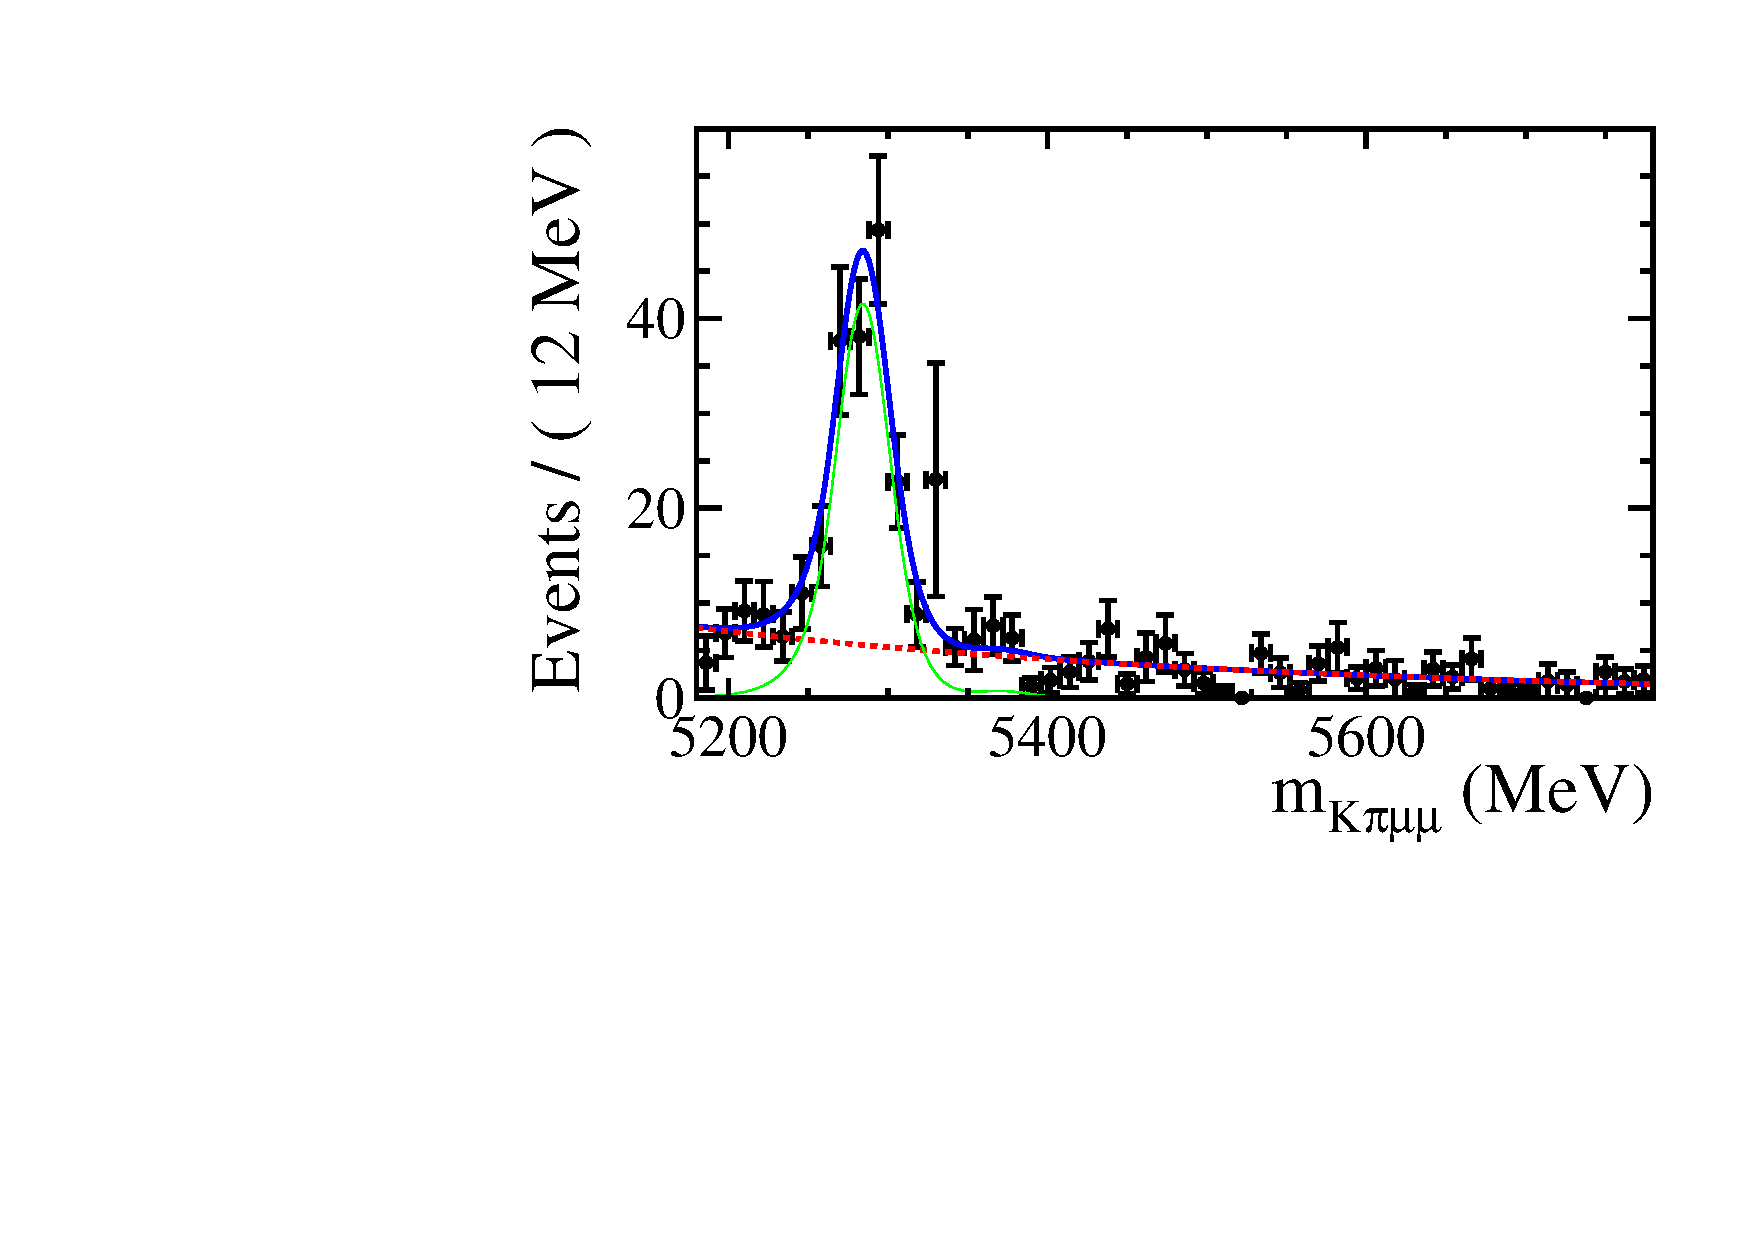
\includegraphics[width=0.45\columnwidth]{chapter7/figs/fits/fit_kstarmumu_swave_mkpi_range_lass_mass_canvas_0.pdf}}
\subfigure[$2.00<\qsq<4.30\gevgevcccc$]{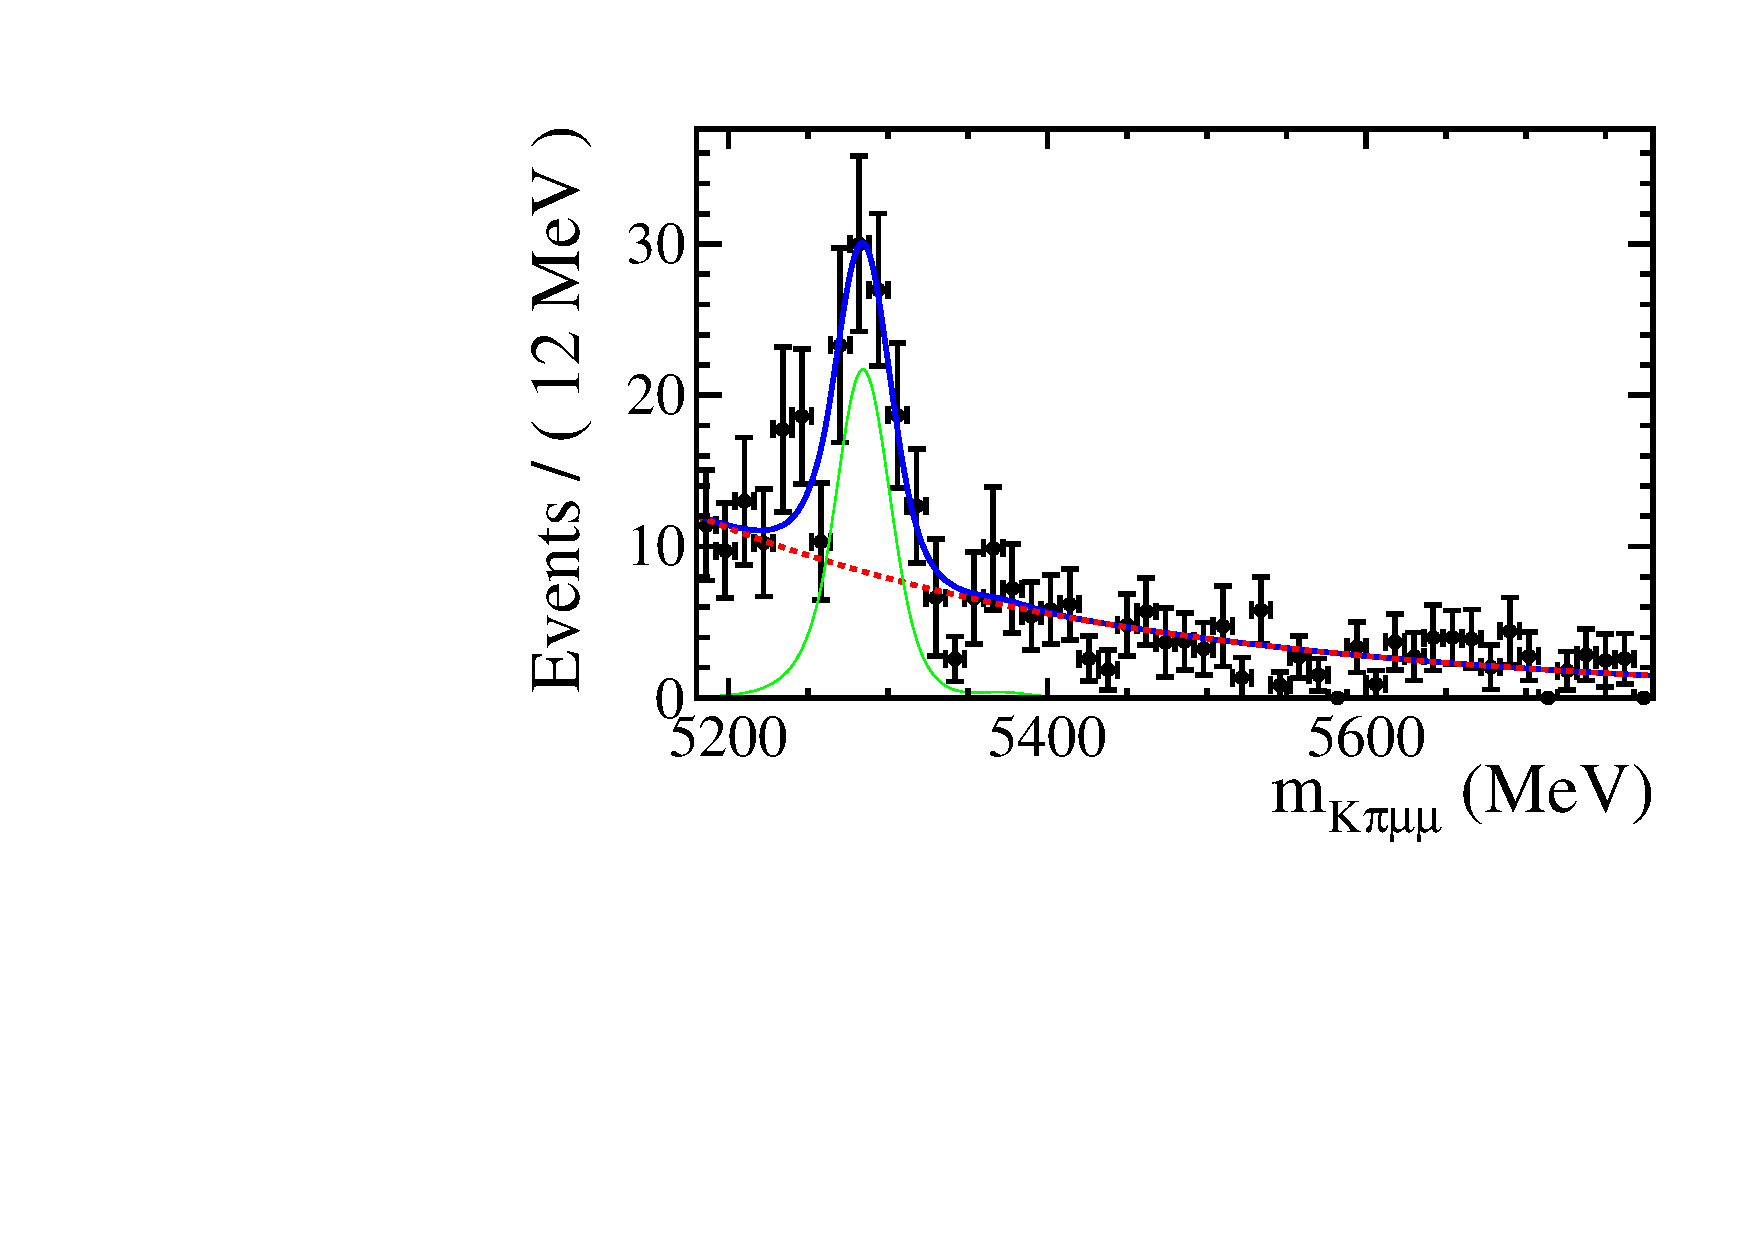
\includegraphics[width=0.45\columnwidth]{chapter7/figs/fits/fit_kstarmumu_swave_mkpi_range_lass_mass_canvas_1.pdf}}
\subfigure[$4.30<\qsq<8.68\gevgevcccc$]{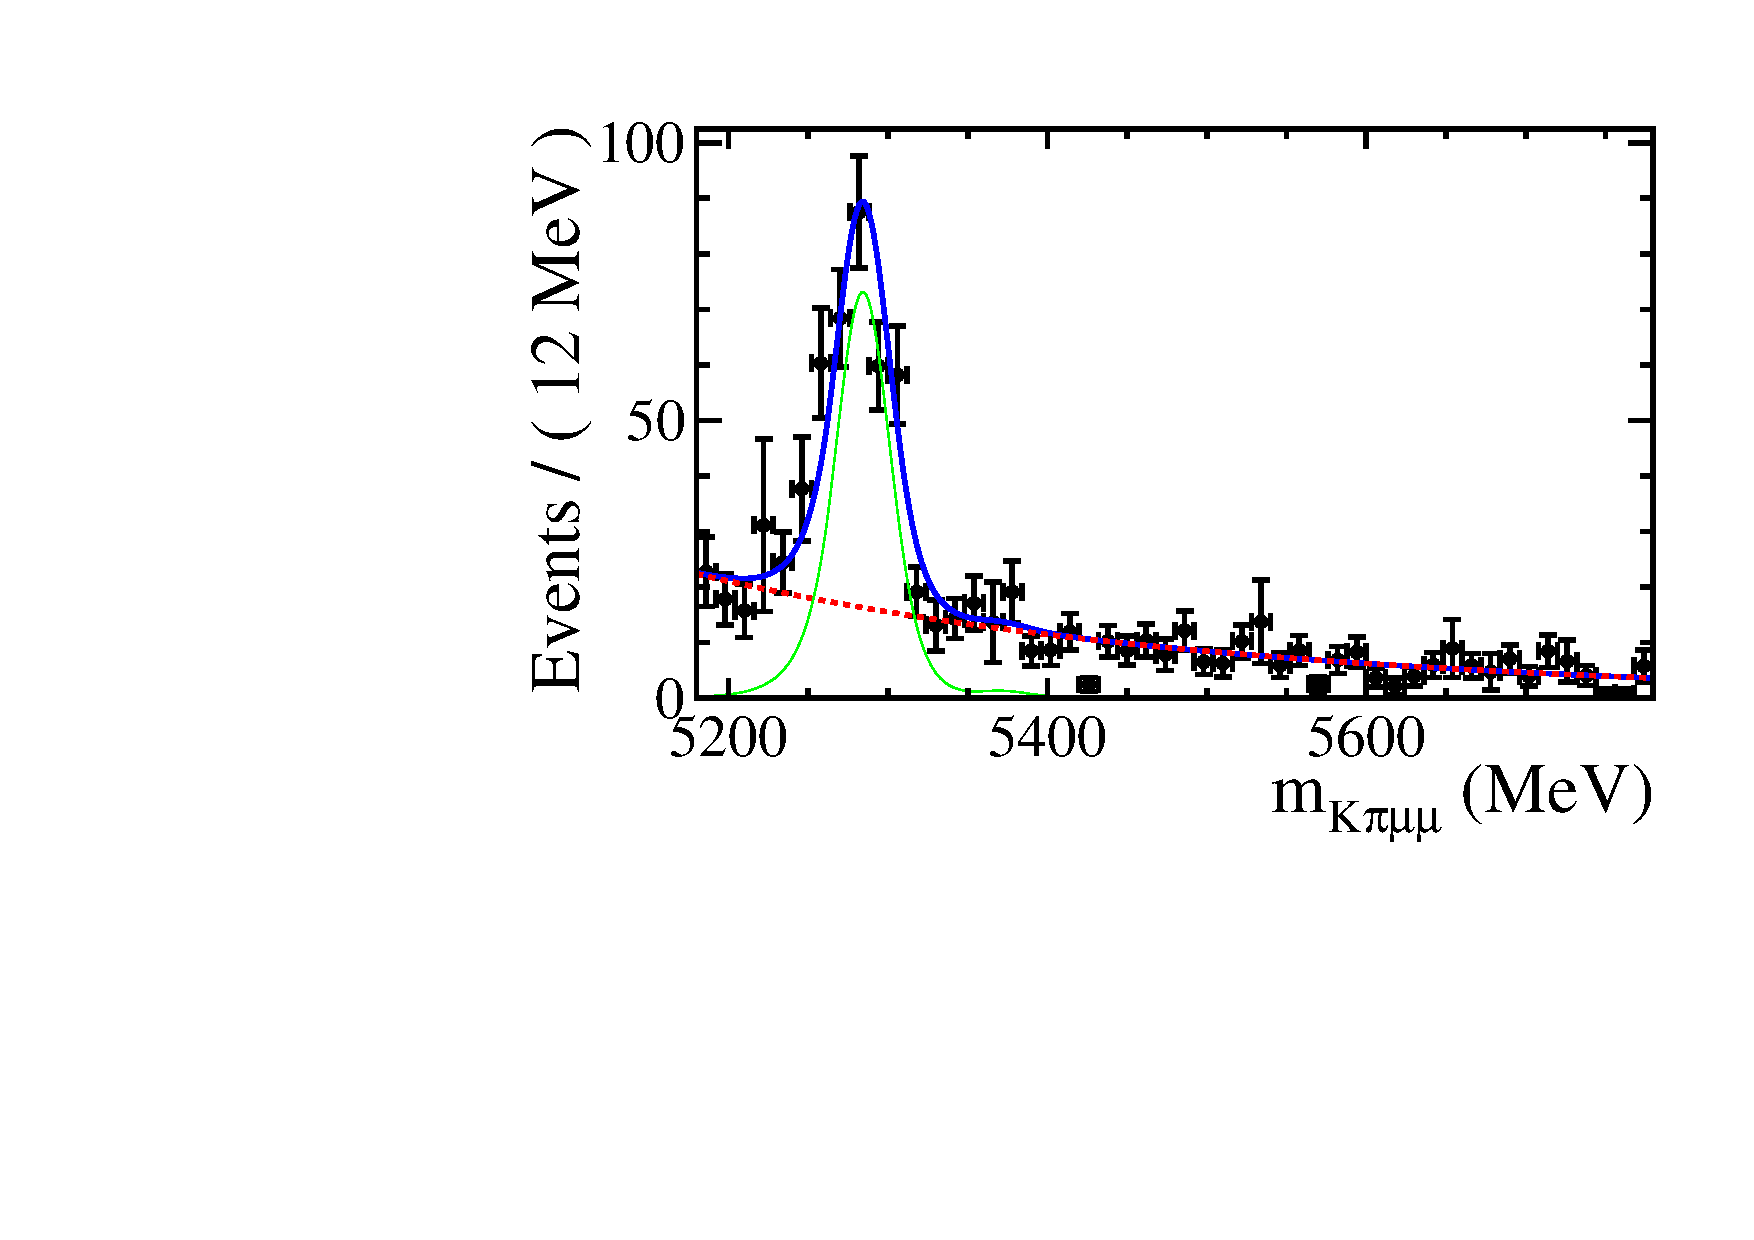
\includegraphics[width=0.45\columnwidth]{chapter7/figs/fits/fit_kstarmumu_swave_mkpi_range_lass_mass_canvas_2.pdf}}
\subfigure[$10.09<\qsq<12.9\gevgevcccc$]{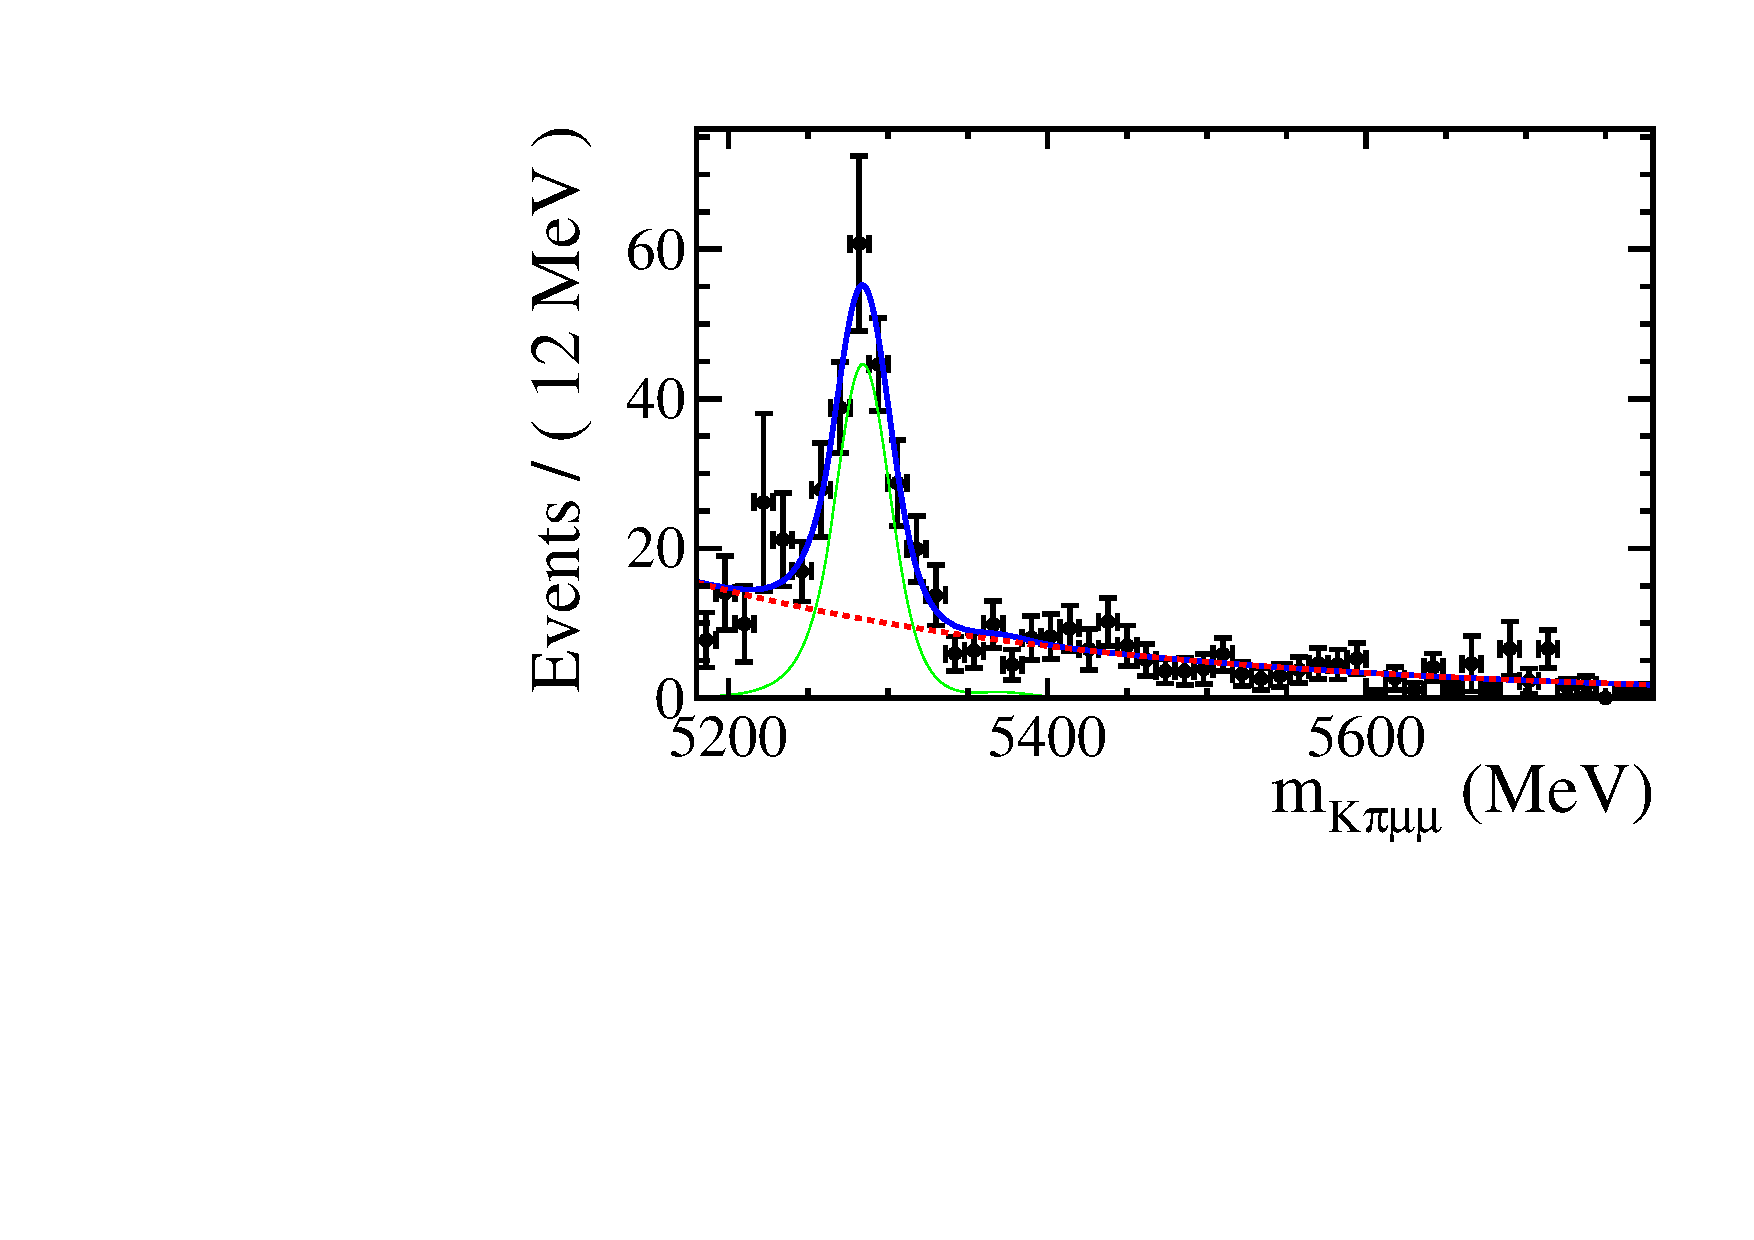
\includegraphics[width=0.48\columnwidth]{chapter7/figs/fits/fit_kstarmumu_swave_mkpi_range_lass_mass_canvas_3.pdf}}
\subfigure[$14.18<\qsq<16.0\gevgevcccc$]{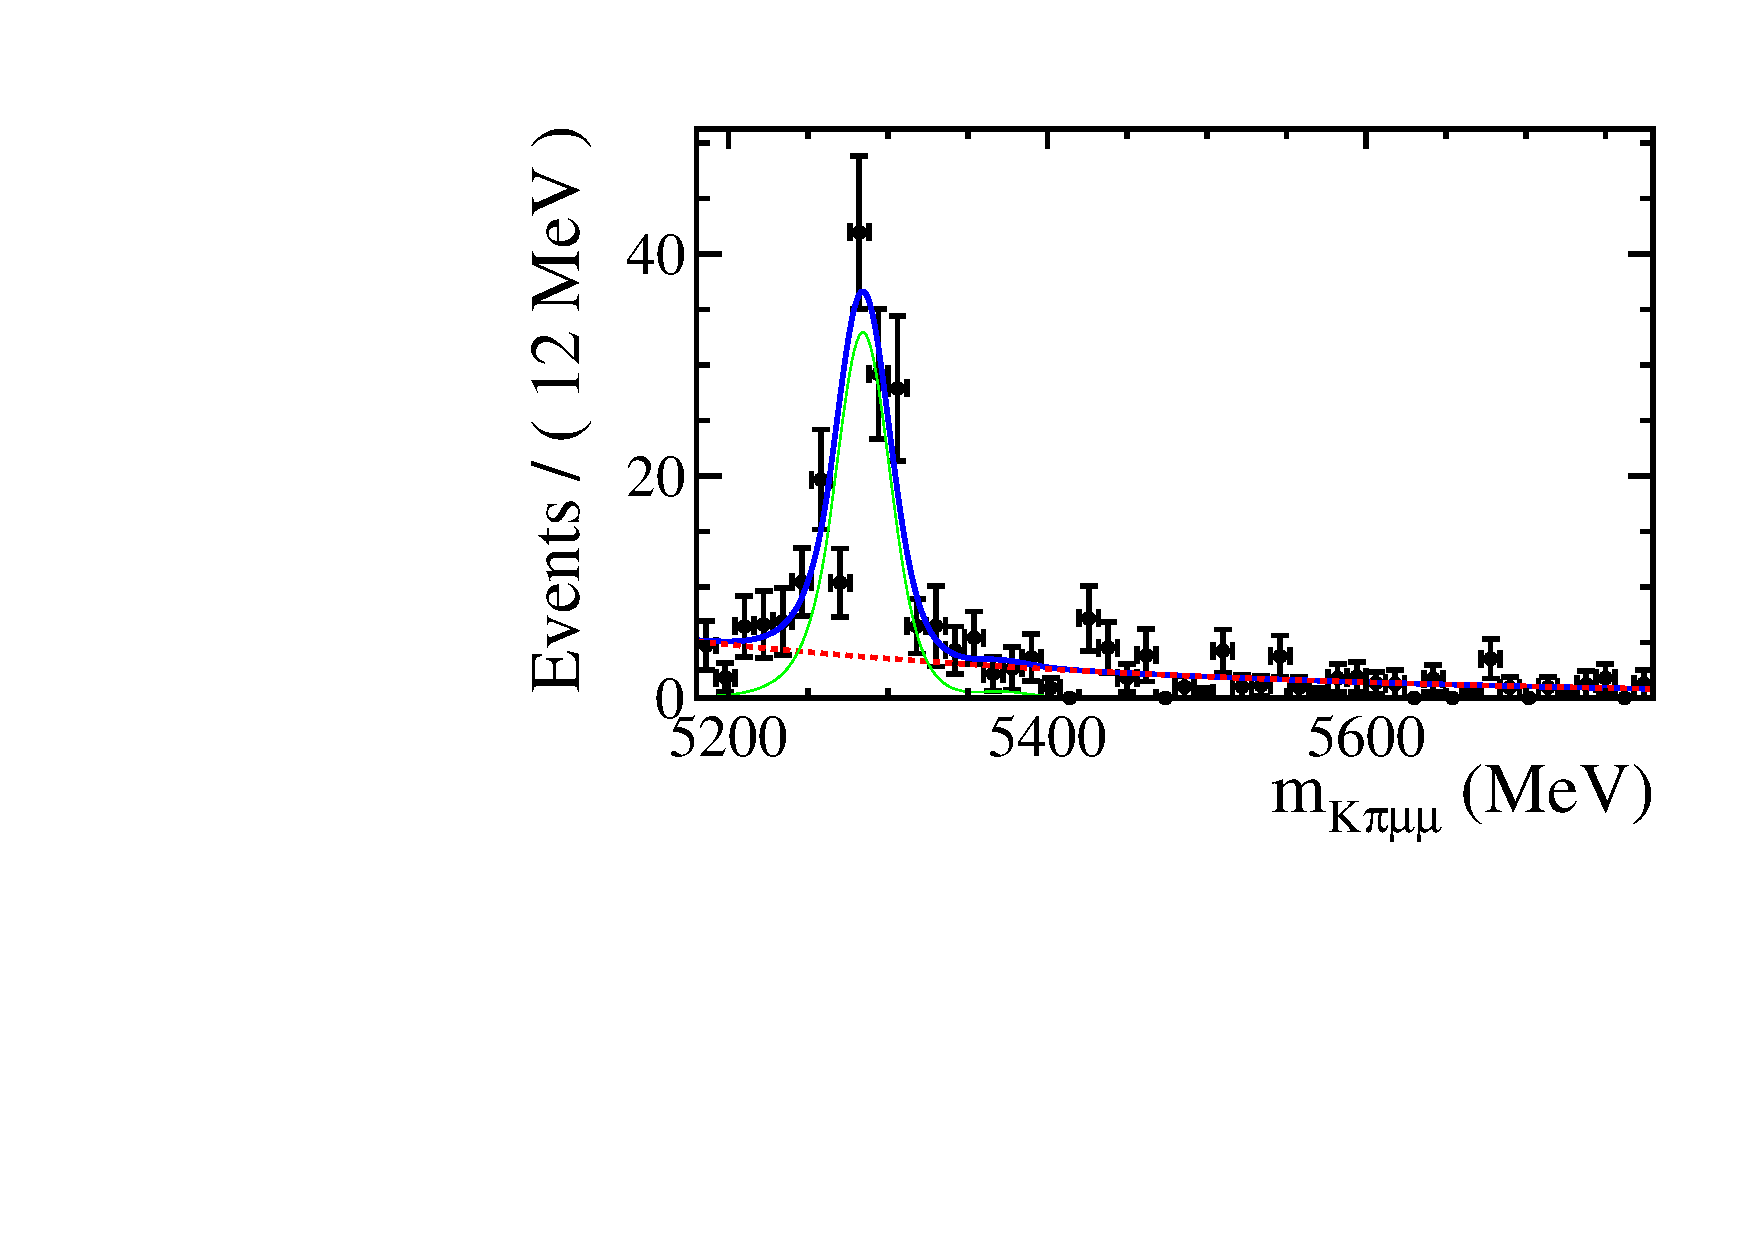
\includegraphics[width=0.45\columnwidth]{chapter7/figs/fits/fit_kstarmumu_swave_mkpi_range_lass_mass_canvas_4.pdf}}
\subfigure[$16.00<\qsq<19.0\gevgevcccc$]{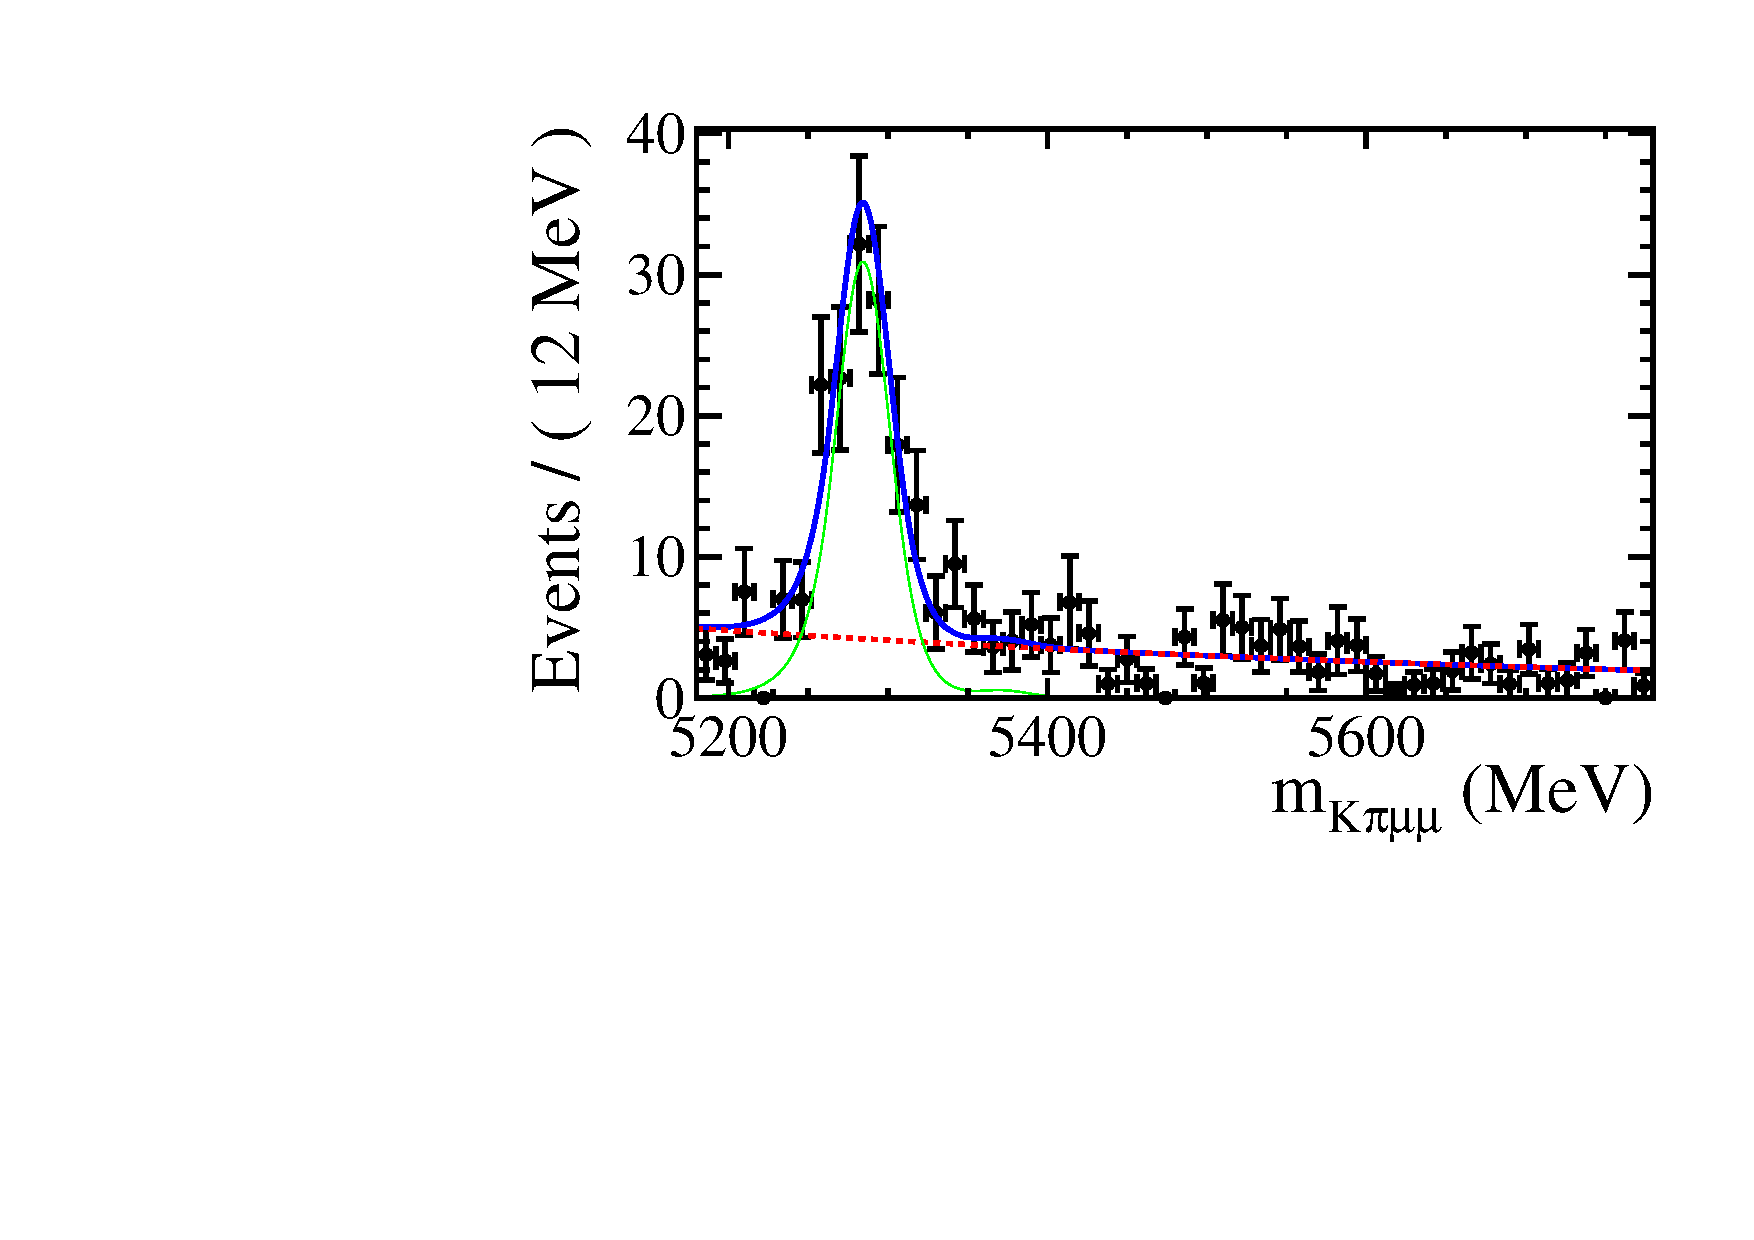
\includegraphics[width=0.45\columnwidth]{chapter7/figs/fits/fit_kstarmumu_swave_mkpi_range_lass_mass_canvas_5.pdf}}
\subfigure[$1.00<\qsq<6.00\gevgevcccc$]{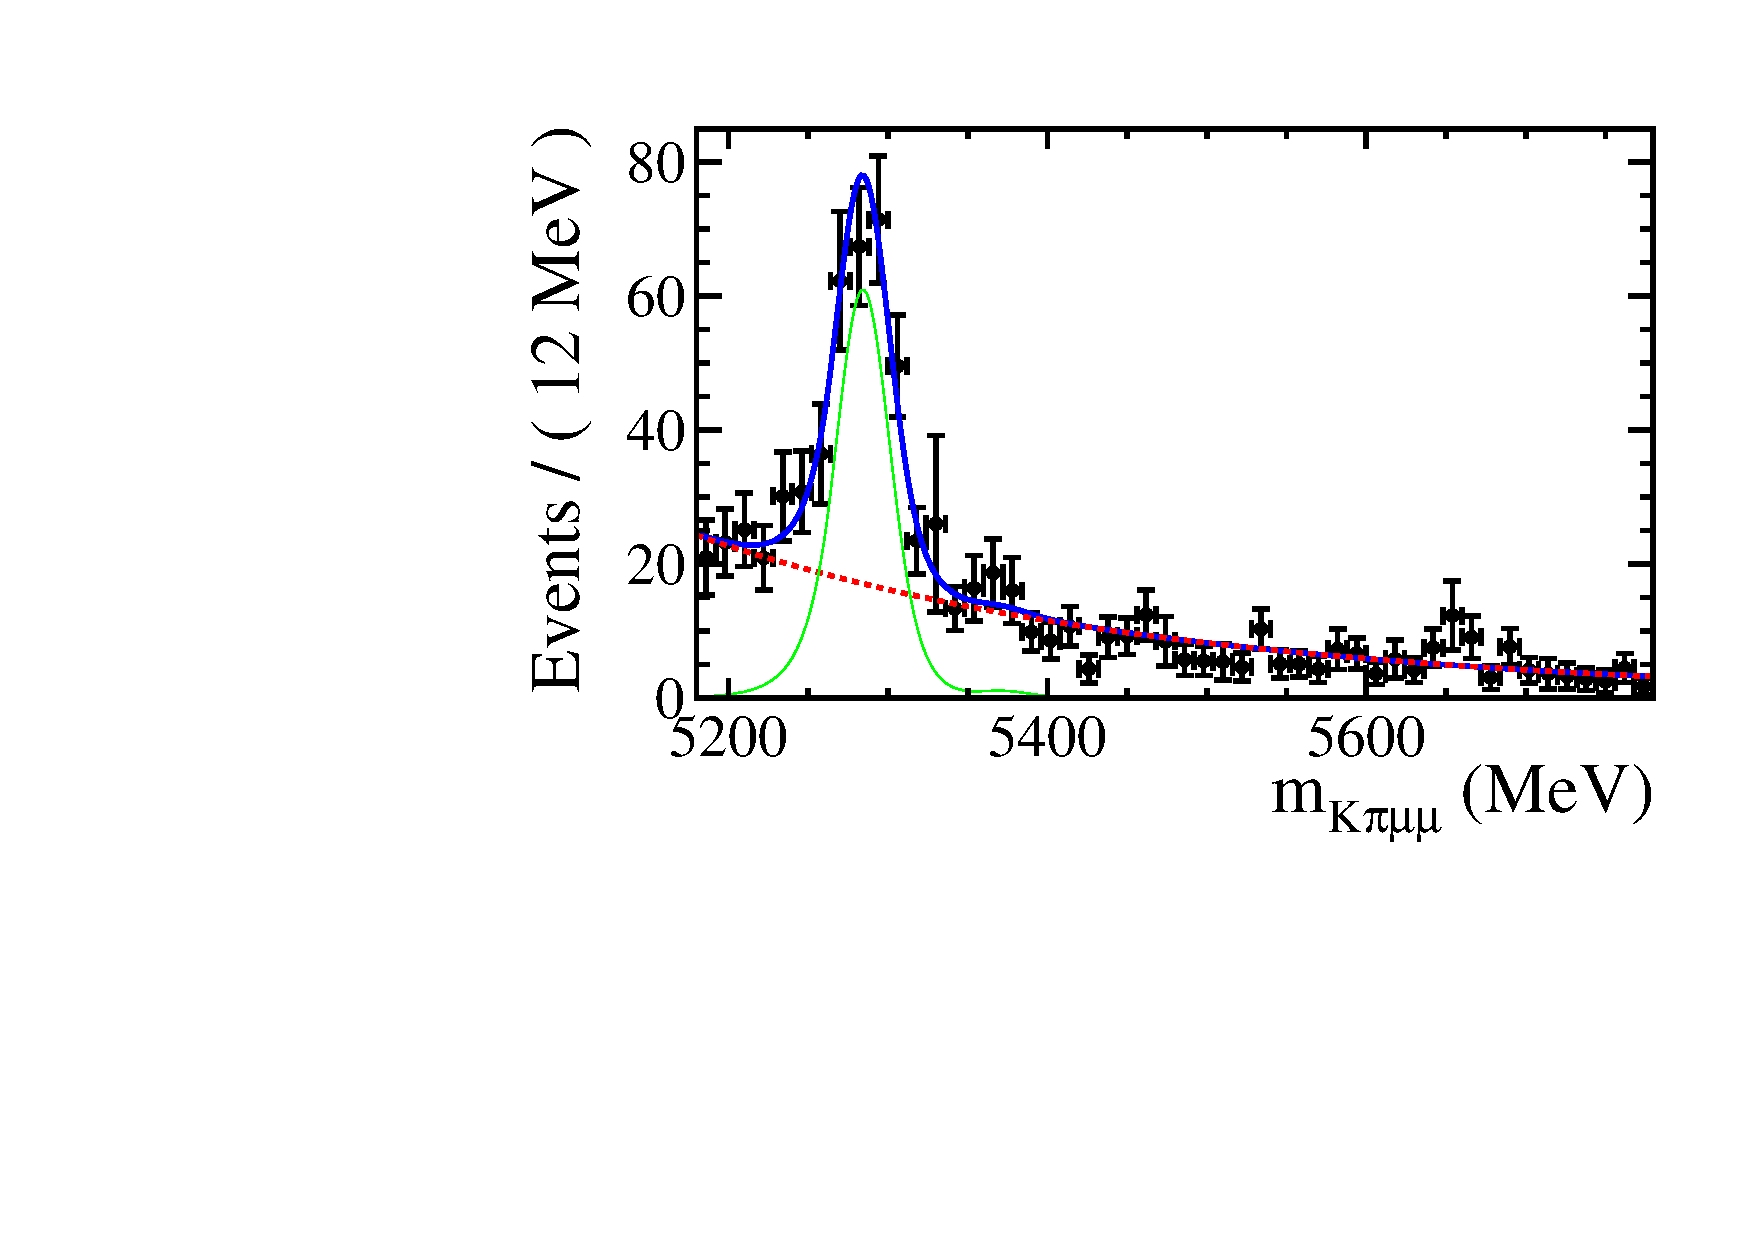
\includegraphics[width=0.45\columnwidth]{chapter7/figs/fits/fit_kstarmumu_swave_mkpi_range_lass_mass_canvas_6.pdf}}
\caption{ The result of the fit to the \kpimm mass spectrum in six \qsq bins for selected \BdToKpimm events from 1.0\invfb of data. ~\label{fig:swave:meas:fits:1} }
\end{figure}
\begin{figure}[tbp]
\centering
\subfigure[$0.10<\qsq<2.00\gevgevcccc$]{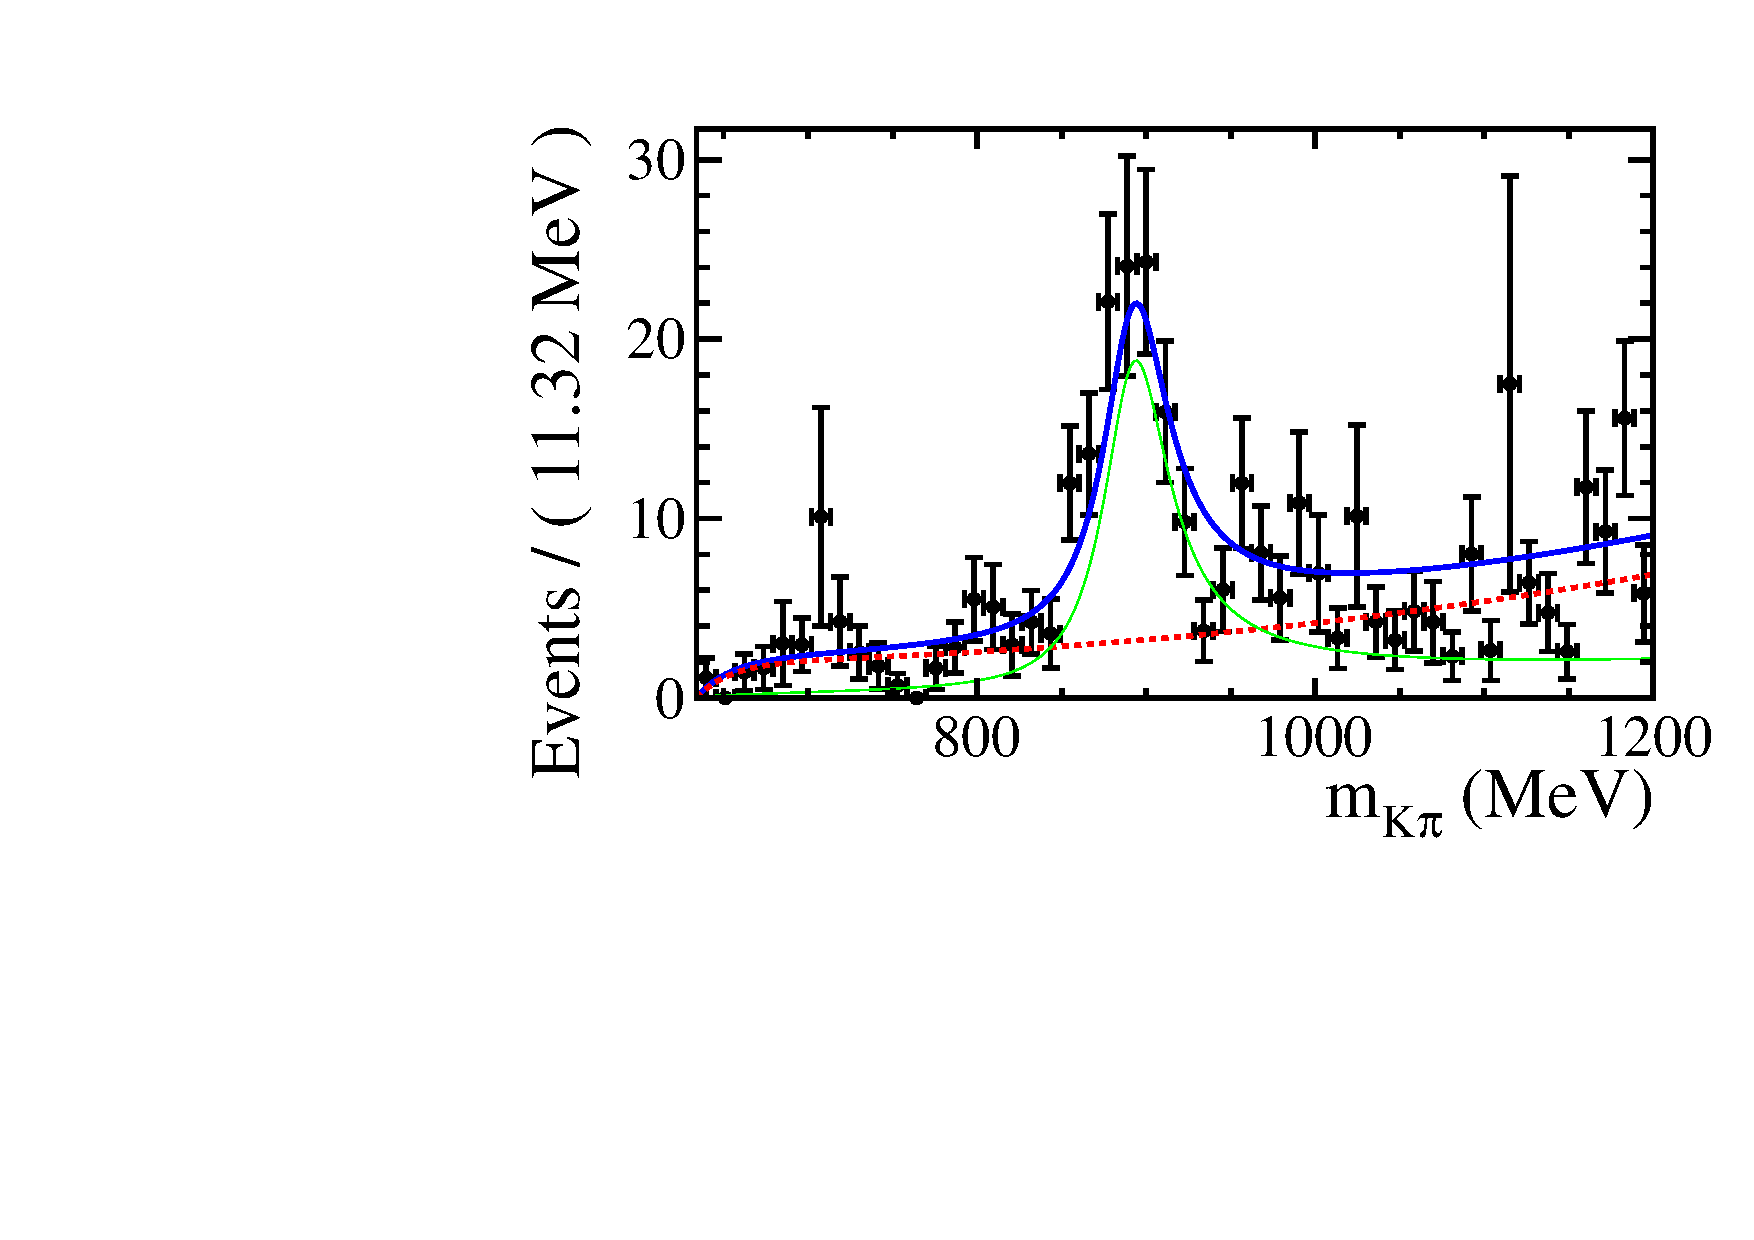
\includegraphics[width=0.45\columnwidth]{chapter7/figs/fits/fit_kstarmumu_swave_mkpi_range_lass_mkpi_canvas_0.pdf}}
\subfigure[$2.00<\qsq<4.30\gevgevcccc$]{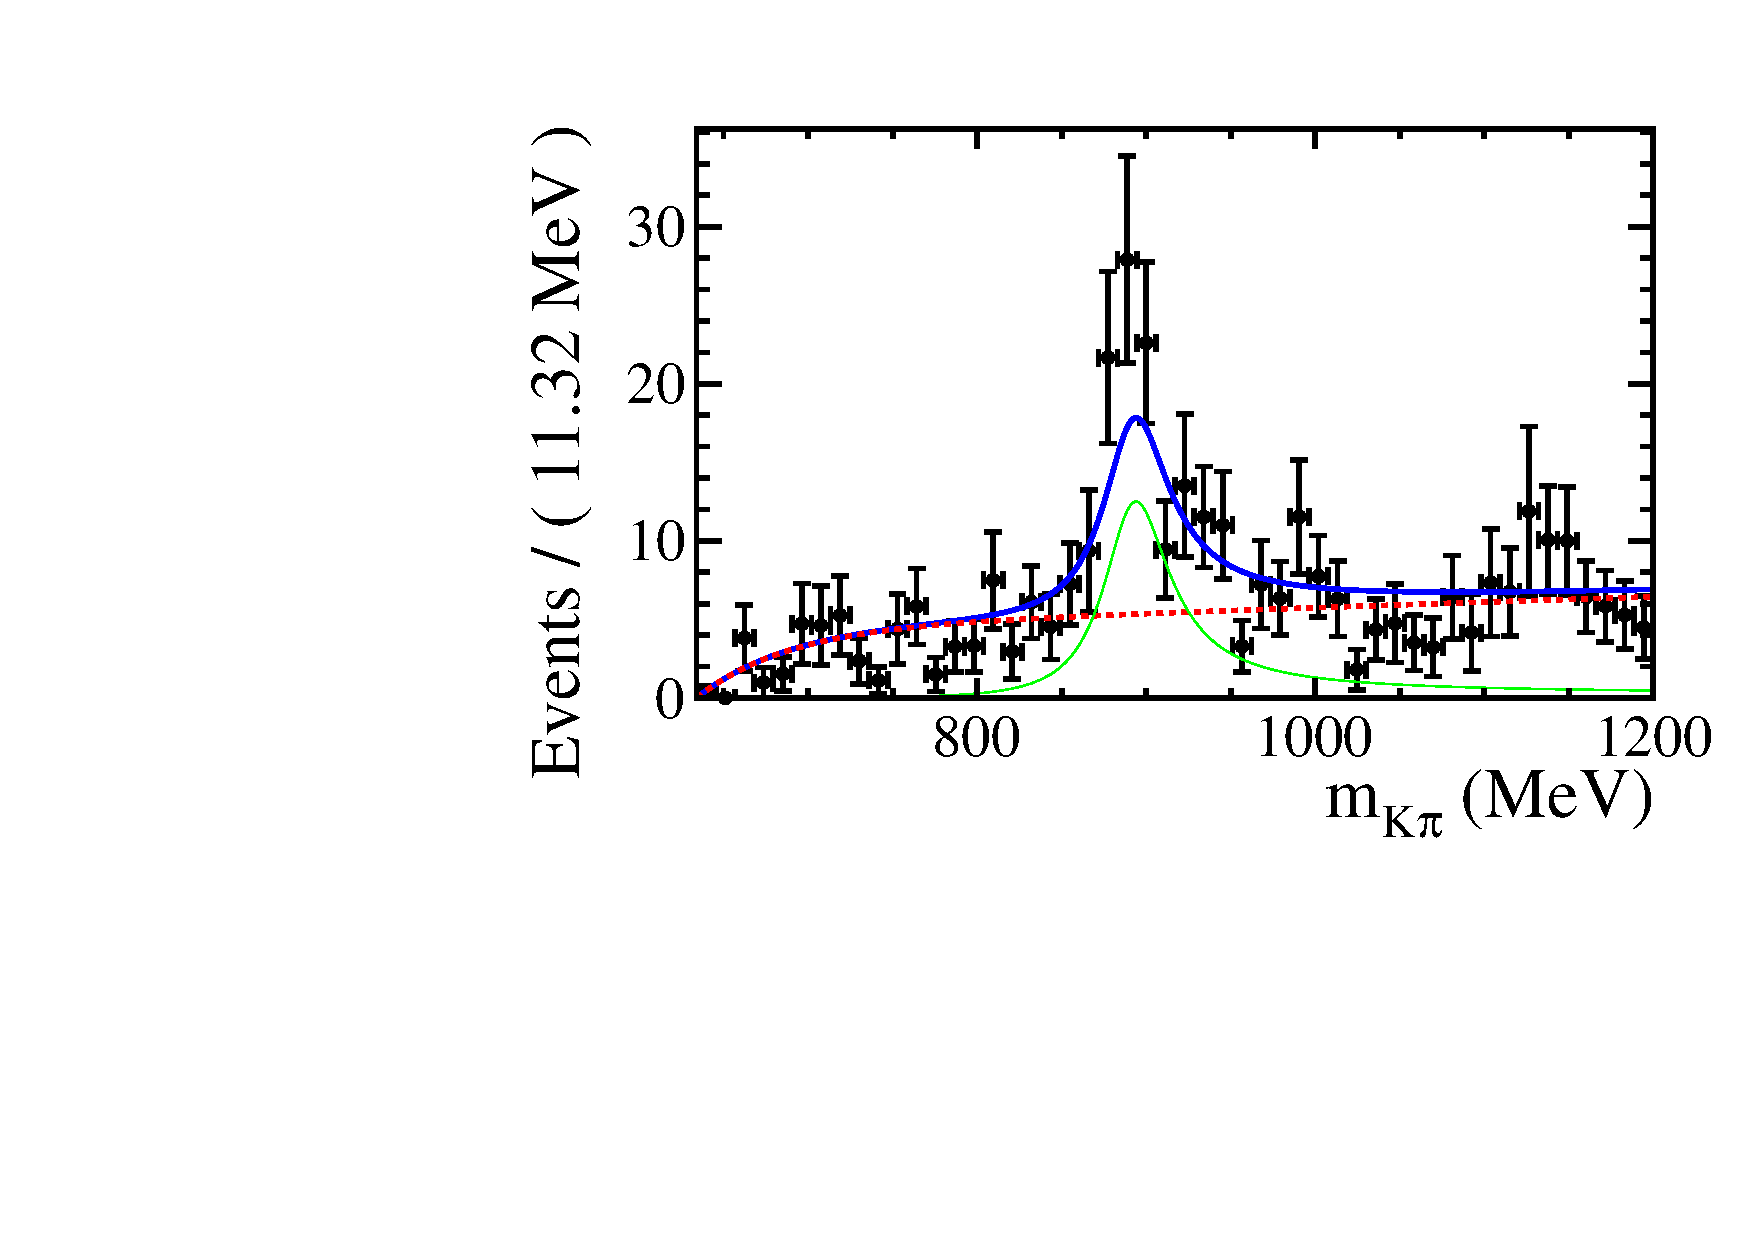
\includegraphics[width=0.45\columnwidth]{chapter7/figs/fits/fit_kstarmumu_swave_mkpi_range_lass_mkpi_canvas_1.pdf}}
\subfigure[$4.30<\qsq<8.68\gevgevcccc$]{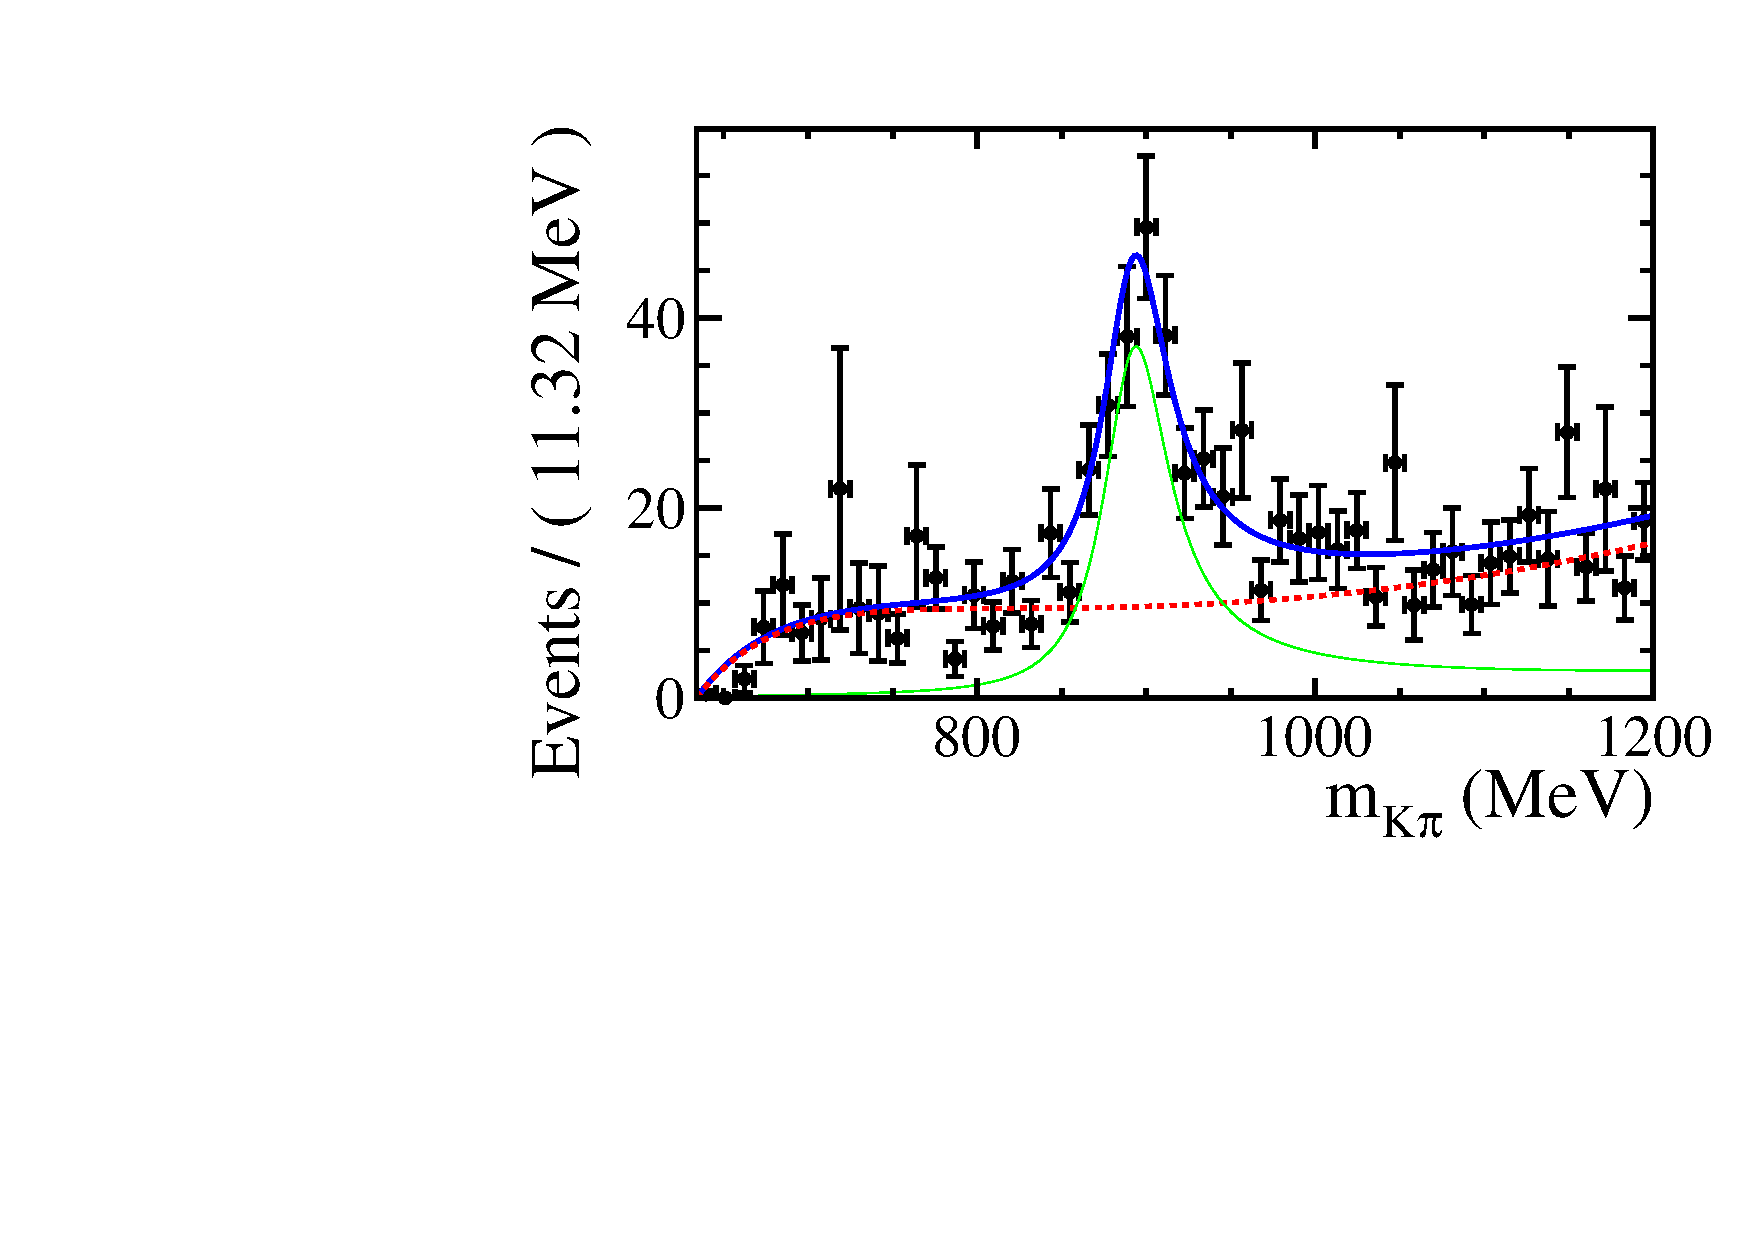
\includegraphics[width=0.45\columnwidth]{chapter7/figs/fits/fit_kstarmumu_swave_mkpi_range_lass_mkpi_canvas_2.pdf}}
\subfigure[$10.09<\qsq<12.9\gevgevcccc$]{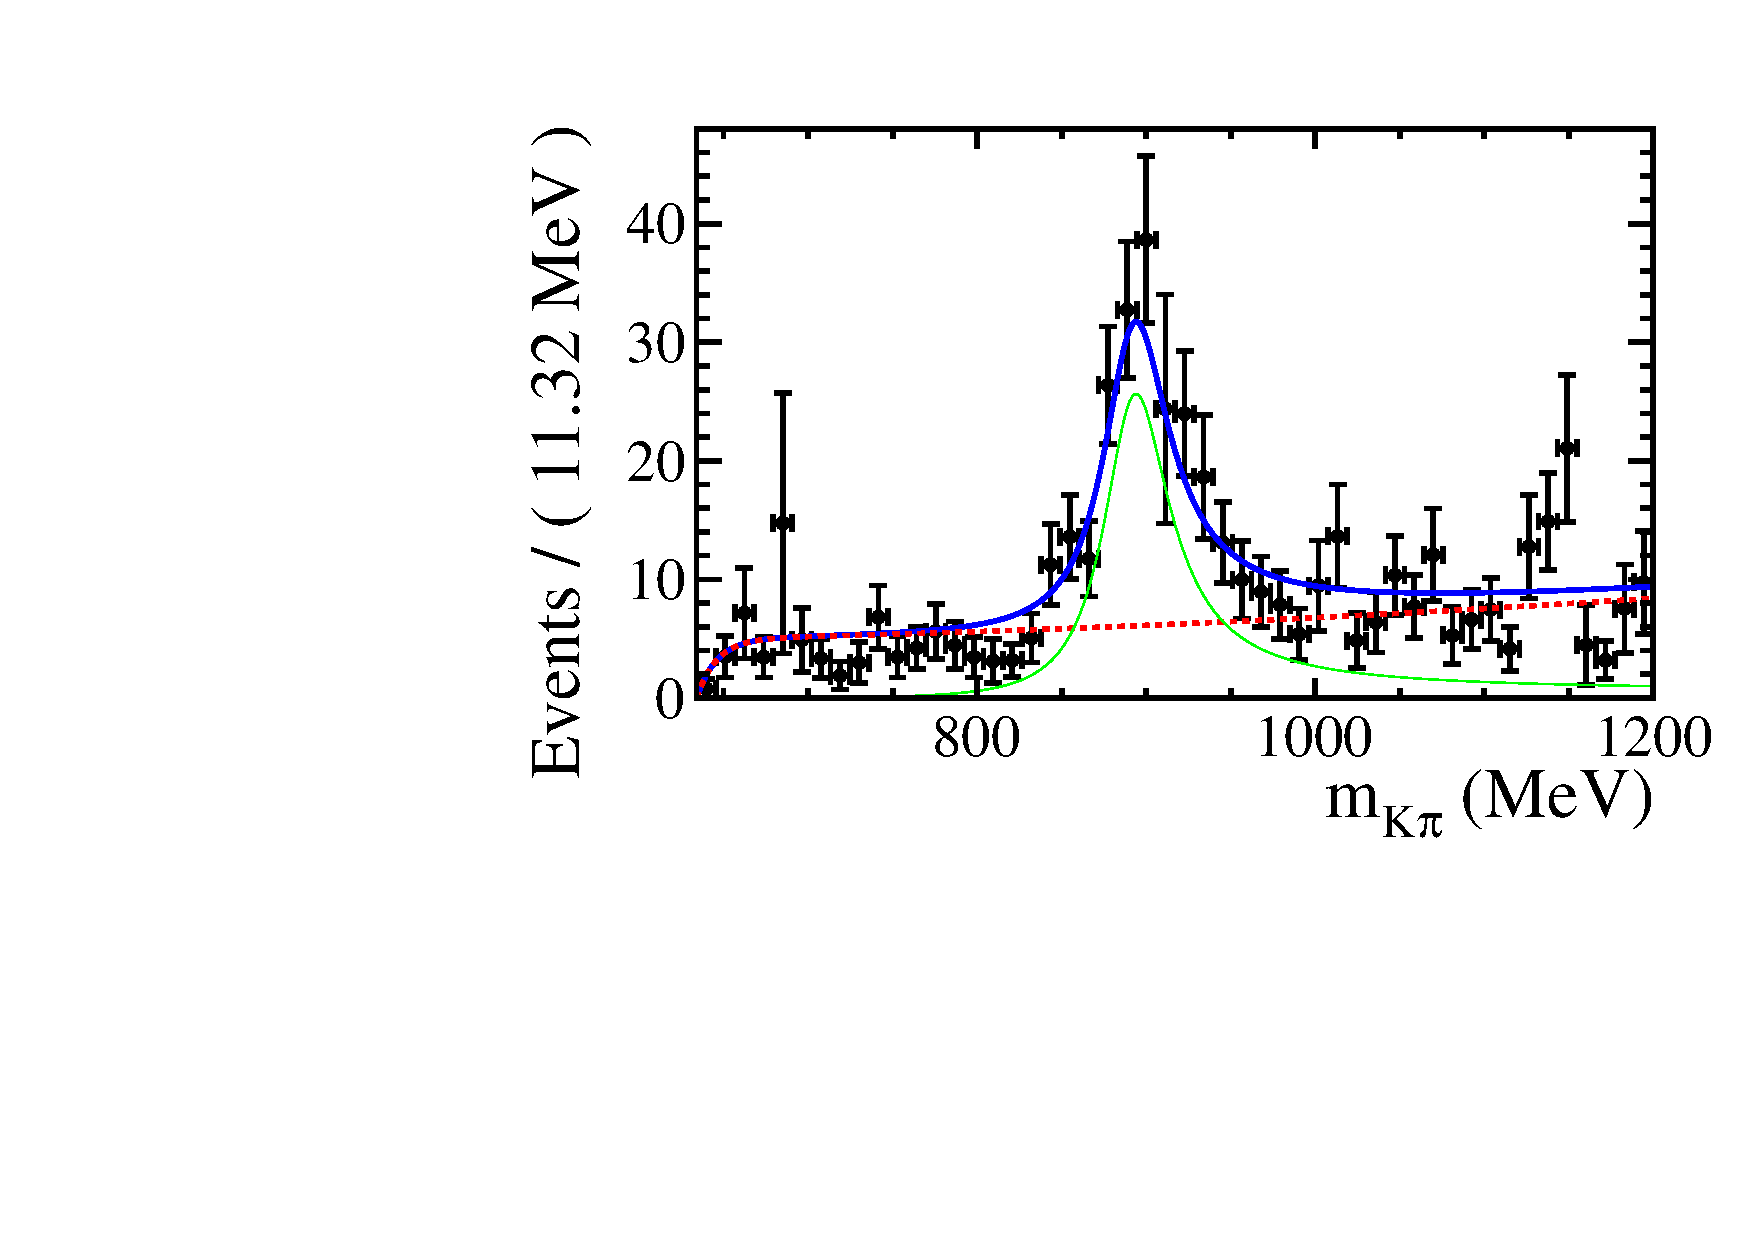
\includegraphics[width=0.45\columnwidth]{chapter7/figs/fits/fit_kstarmumu_swave_mkpi_range_lass_mkpi_canvas_3.pdf}}
\subfigure[$14.18<\qsq<16.0\gevgevcccc$]{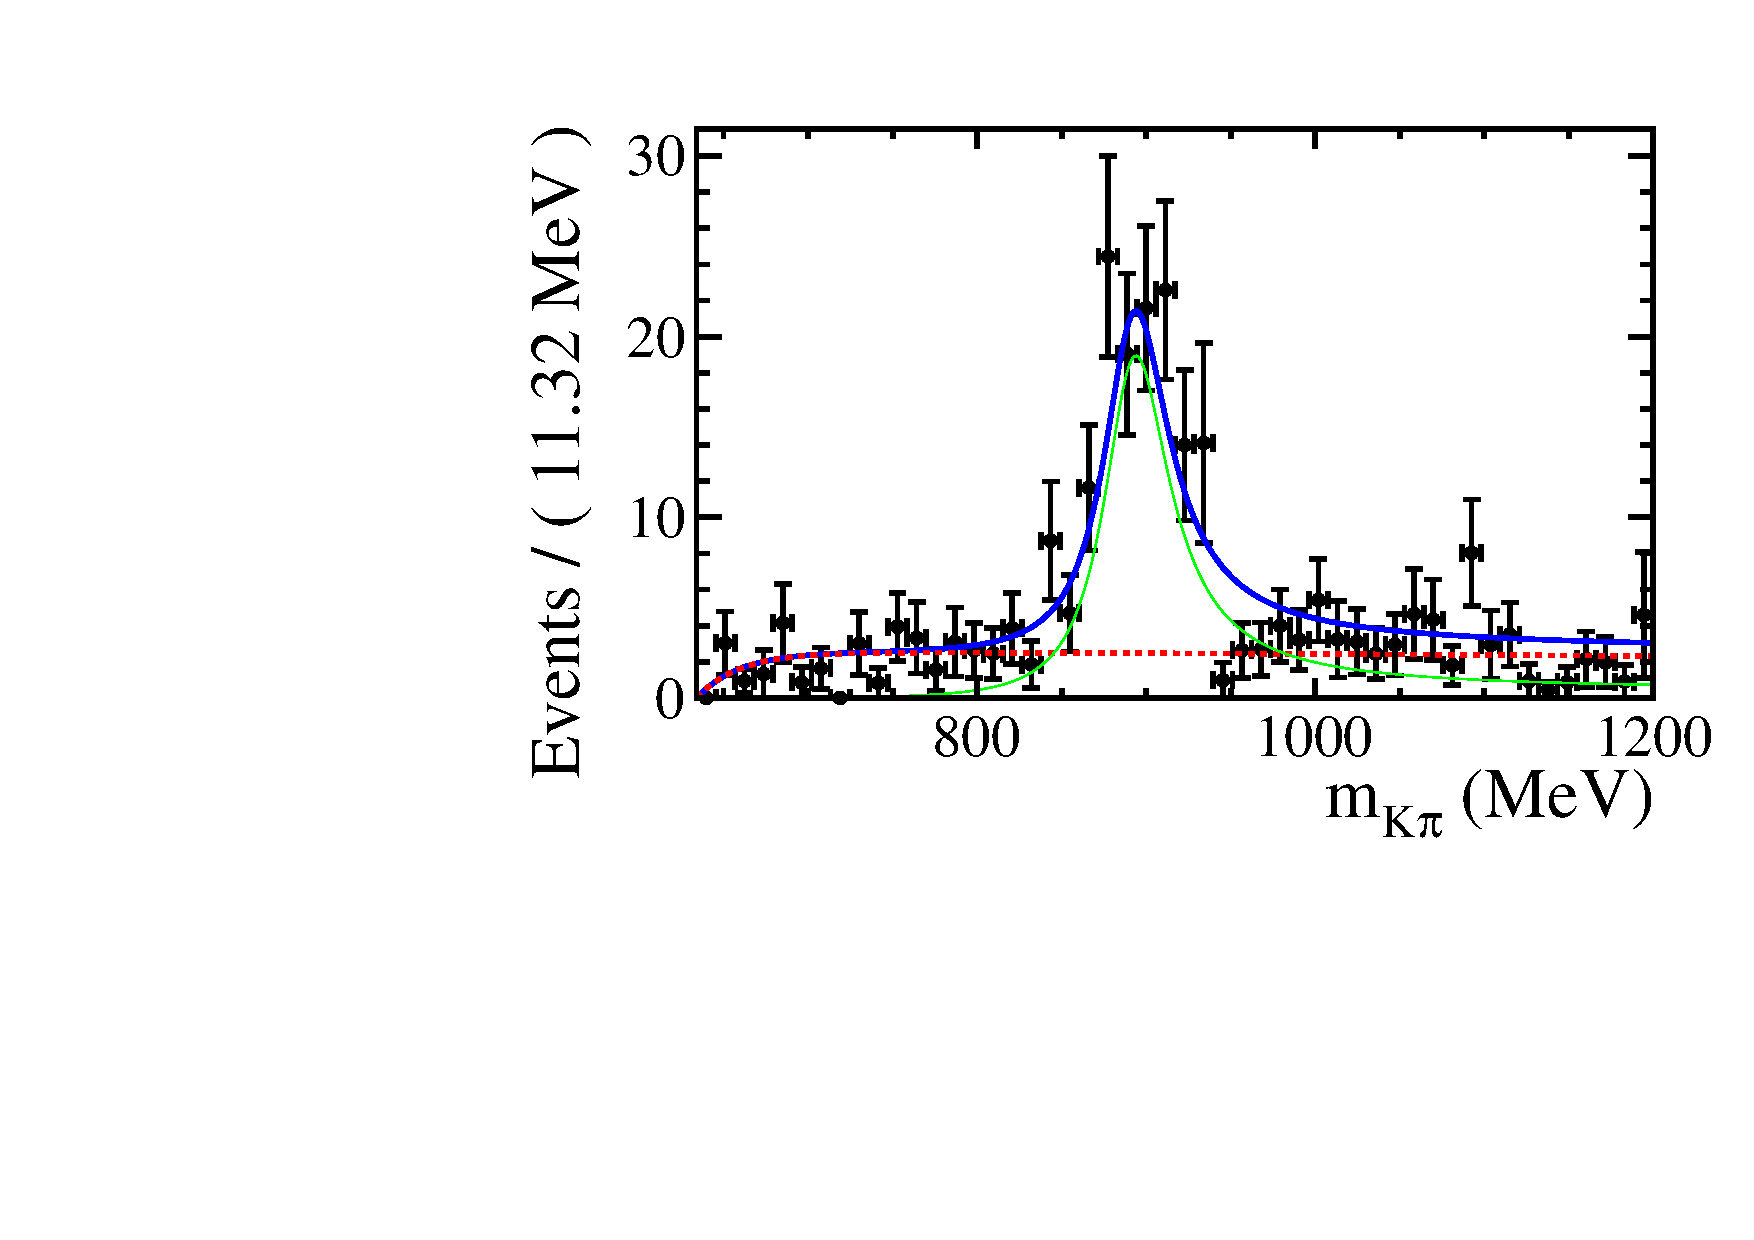
\includegraphics[width=0.45\columnwidth]{chapter7/figs/fits/fit_kstarmumu_swave_mkpi_range_lass_mkpi_canvas_4.pdf}}
\subfigure[$16.0<\qsq<19.0\gevgevcccc$]{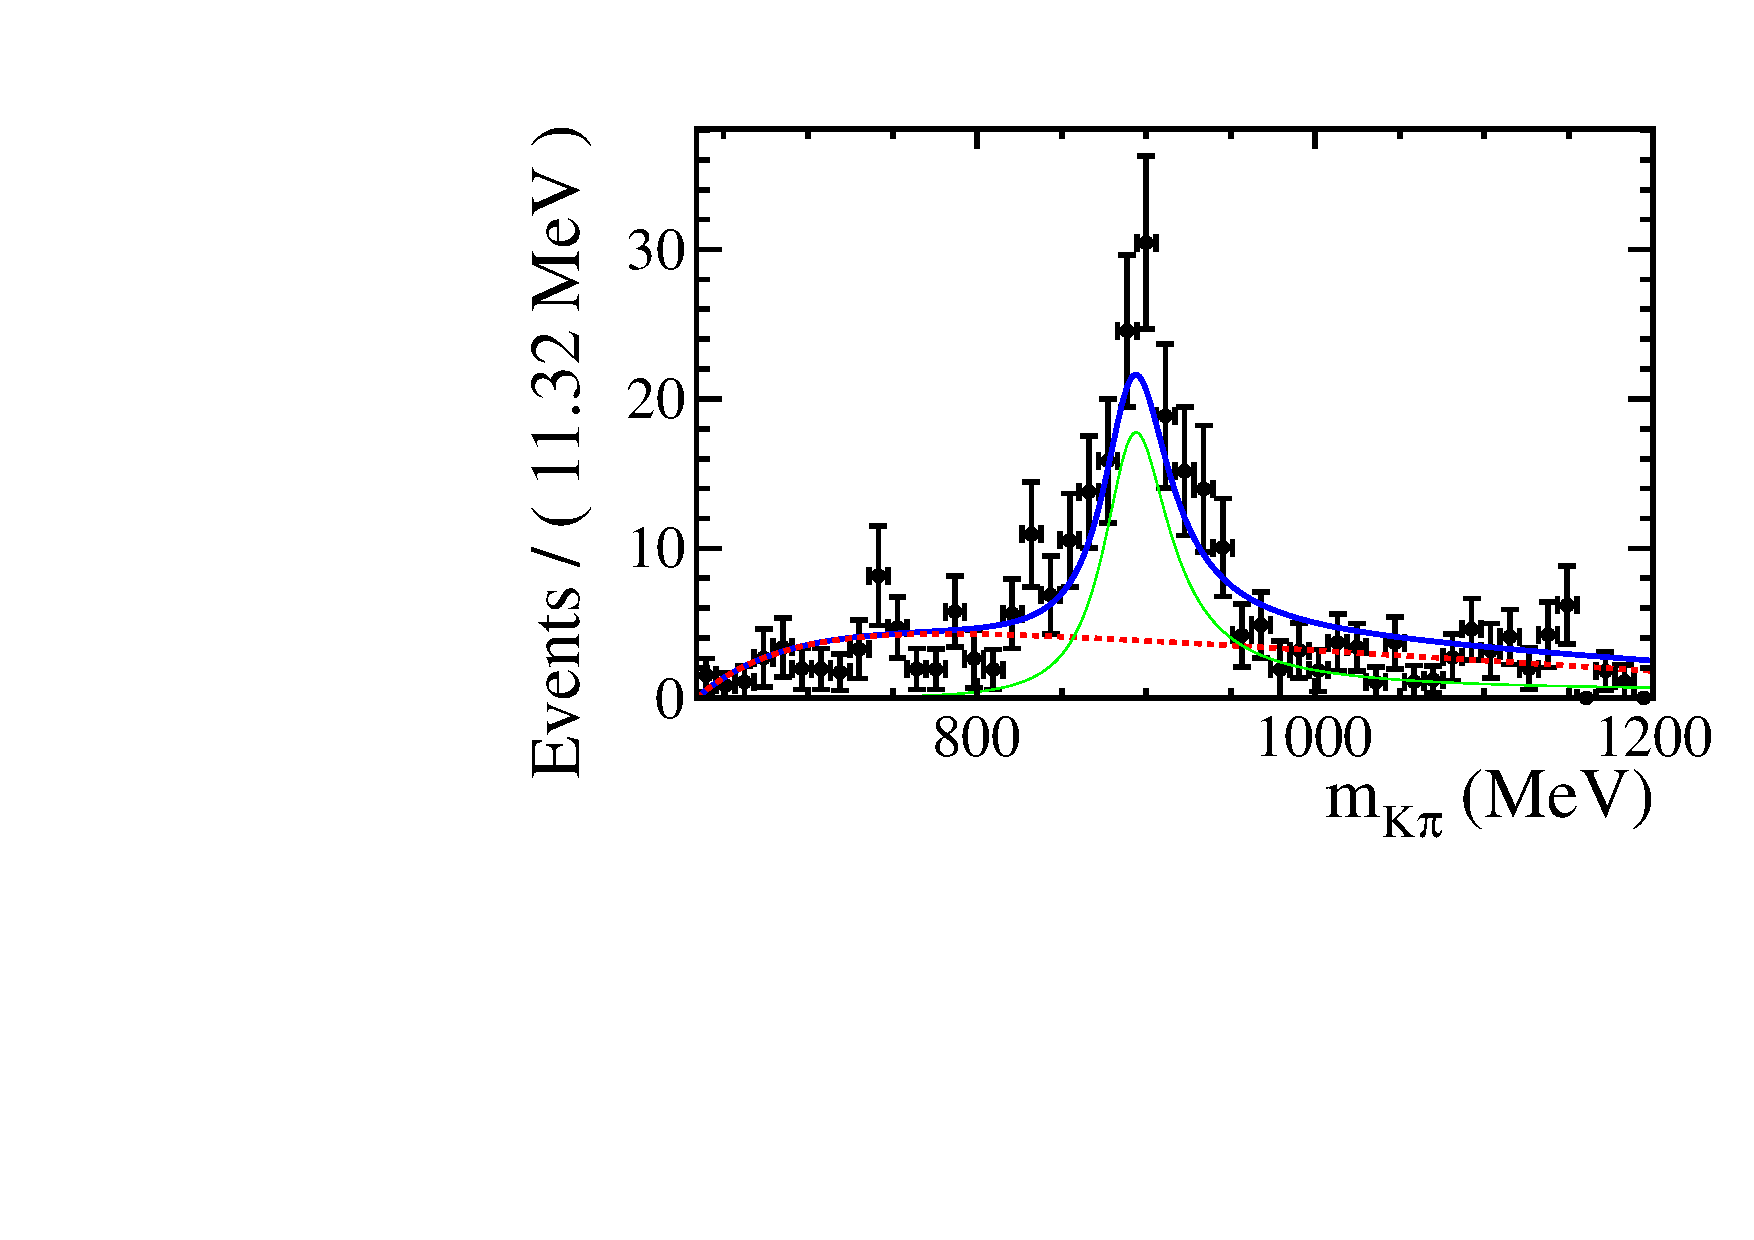
\includegraphics[width=0.45\columnwidth]{chapter7/figs/fits/fit_kstarmumu_swave_mkpi_range_lass_mkpi_canvas_5.pdf}}
\subfigure[$1.00<\qsq<6.00\gevgevcccc$]{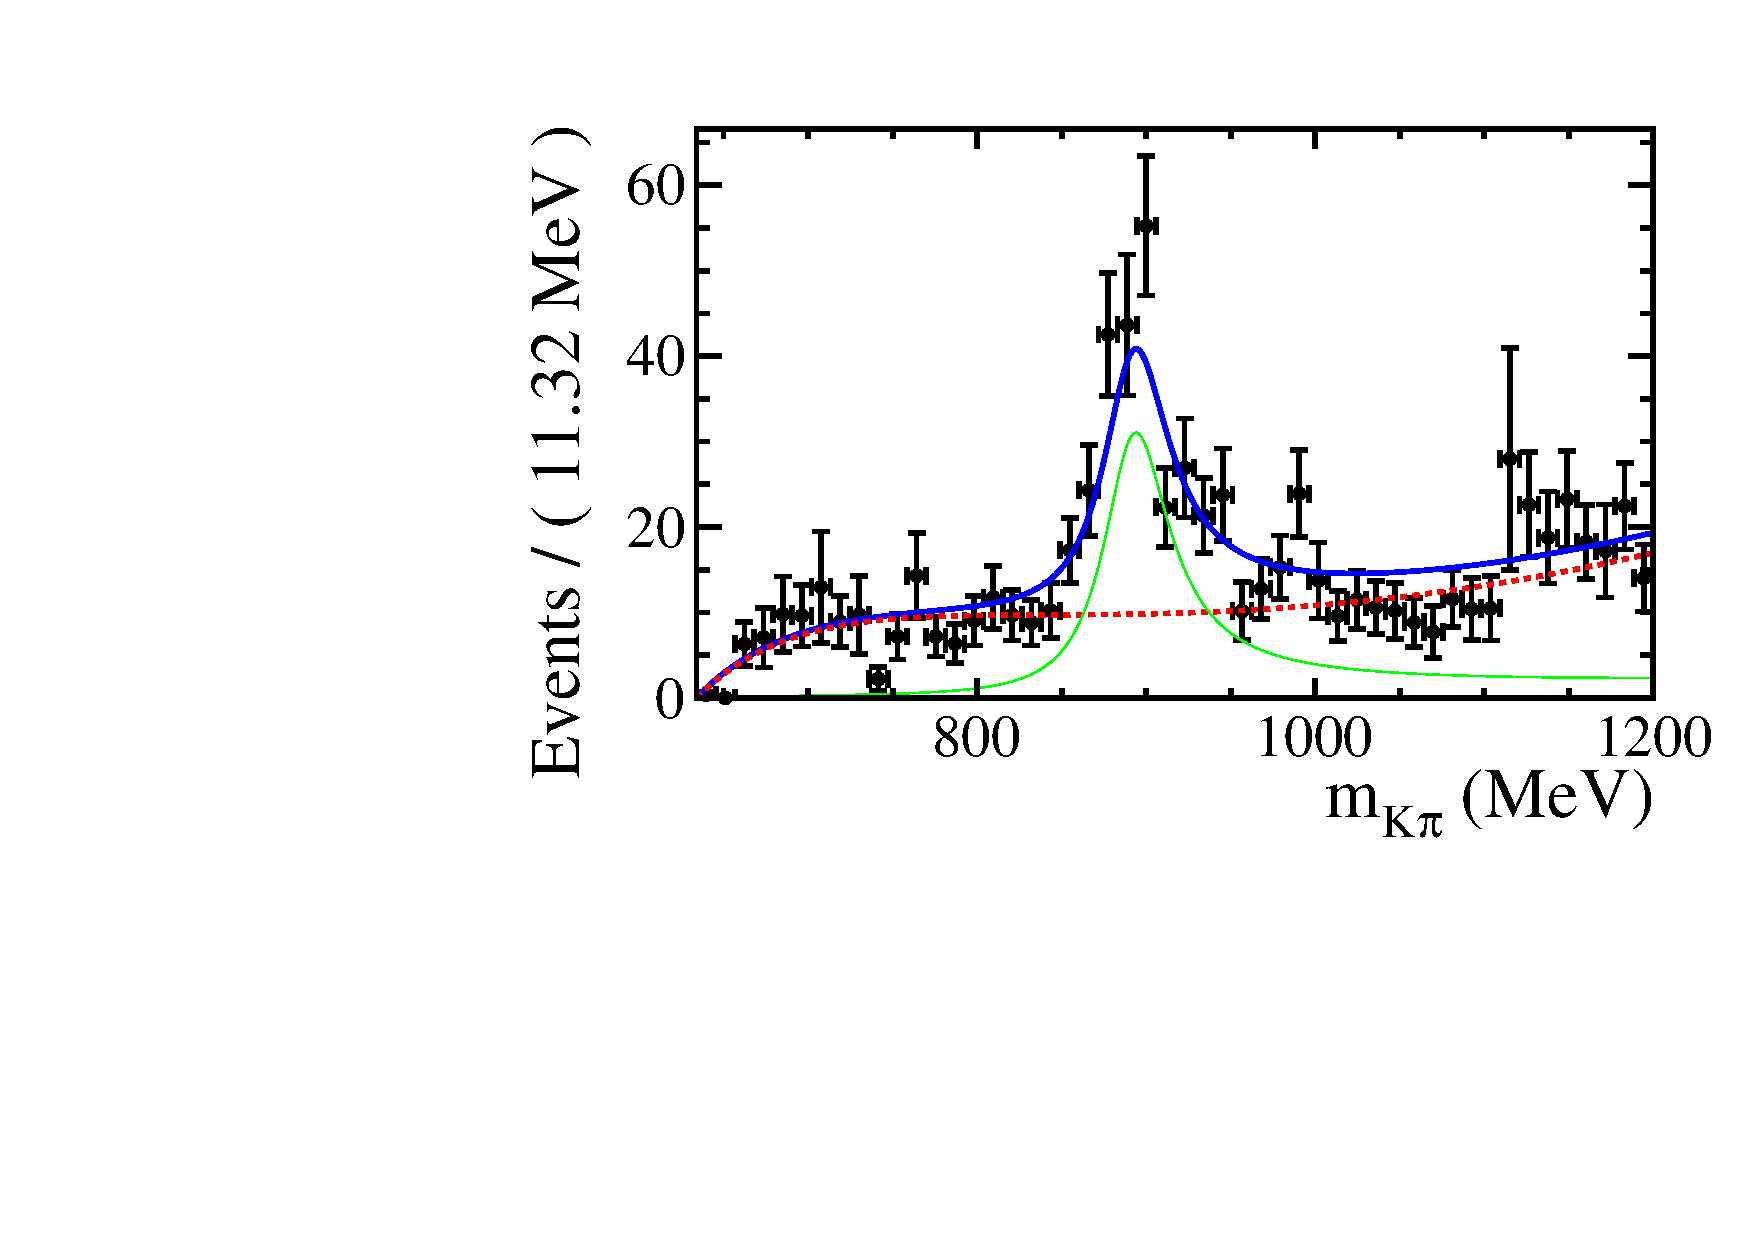
\includegraphics[width=0.45\columnwidth]{chapter7/figs/fits/fit_kstarmumu_swave_mkpi_range_lass_mkpi_canvas_6.pdf}}
\caption{ The results of the fit to the \kpi mass spectrum for selected \BdToKpimm events from 1.0\invfb of data. ~\label{fig:swave:meas:fits:2} }
\end{figure}
The results of the measurement of the \kpi S-wave in \BdToKpimm using 1.0\invfb of integrated luminosity collected at \lhcb are presented in Fig.~\ref{fig:swave:meas:results}.
\begin{figure}[tbp]
\centering
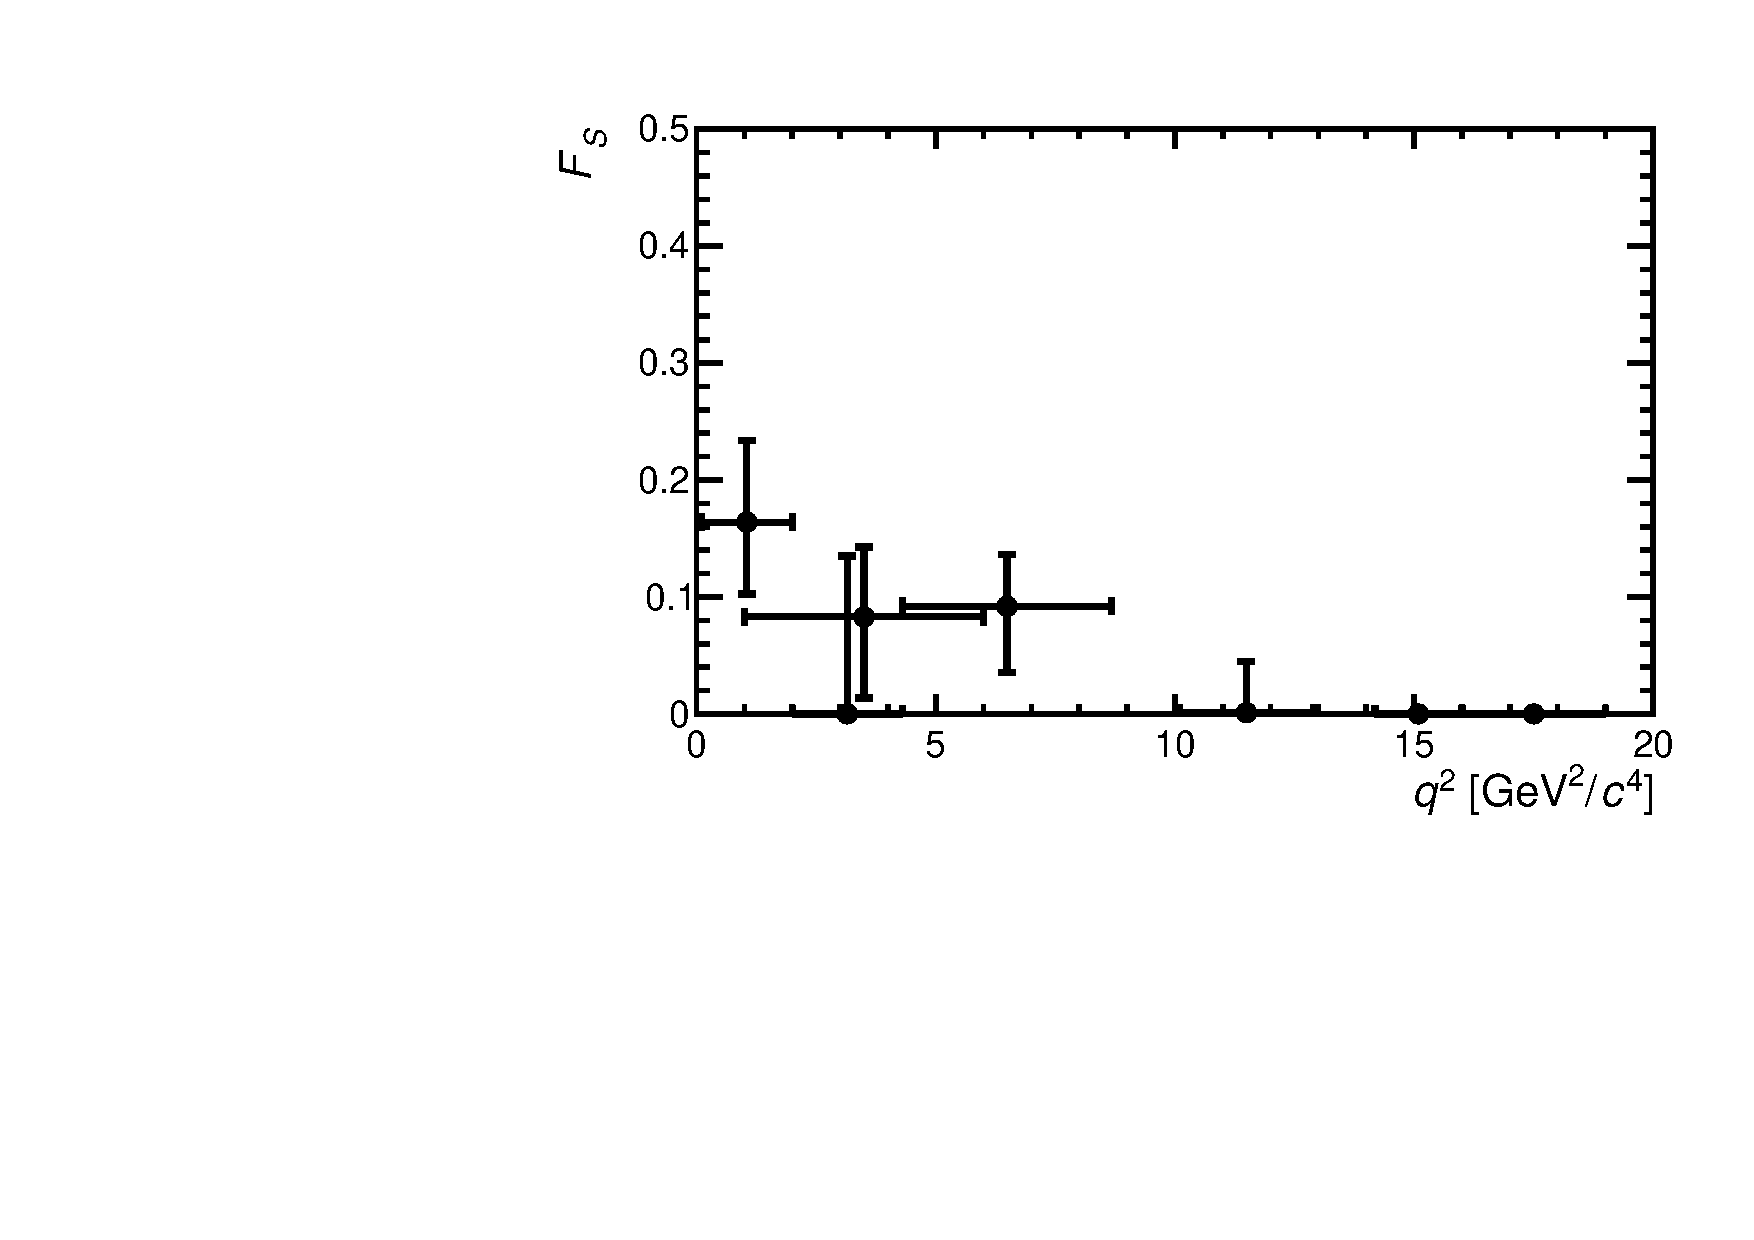
\includegraphics[width=0.66\columnwidth]{chapter7/figs/fits/plot_swave_FS.pdf}
\caption[ The fraction of \kpi S-wave in six bins of \qsq for selected \BdToKpimm 
events from 1.0\invfb of data collected at $\sqs=7\tev$ at \lhcb in 2011.   ]
{ The fraction of \kpi S-wave in six bins of \qsq for selected \BdToKpimm 
events from 1.0\invfb of data collected at $\sqs=7\tev$ at \lhcb in 2011.
For the regions where no S-wave is found, the upper error bar indicates the 95\% confidence limit.
~\label{fig:swave:meas:results} }
\end{figure}
The central values, statistical and systematic errors in 6 bins of \qsq are given in Table~\ref{tbl:swave:results}.
\setlength\extrarowheight{3pt}
\begin{table}[tbp]
\centering
\caption[ Table showing the fraction of \kpi S-wave in six bins of \qsq for selected \BdToKpimm 
events from 1.0\invfb of data collected at $\sqs=7\tev$ at \lhcb in 2011.    ]
{ Table showing the fraction of \kpi S-wave between 0.64<\psq<1.00 in six bins of \qsq for selected \BdToKpimm 
events from 1.0\invfb of data collected at $\sqs=7\tev$ at \lhcb in 2011.
For the regions where no S-wave is found, results are quoted at 95\% confidence limit.
~\label{tbl:swave:results} }
\begin{tabular}{|c|c|}
\hline
Bin (\gevgevcccc) & \FS \\ 
\hline
 $ 0.10<\qsq< 2.00$   & $0.164_{-0.060}^{-0.069}~_{+0.013}^{-0.011} $\\ 
 $ 2.00 <\qsq<  4.30$  & $ < 0.135~(\mathrm{at~95\%~C.L.}) $\\ 
 $ 4.30 <\qsq<  8.68$  & $0.092_{-0.033}^{-0.039}~_{+0.046}^{-0.021} $\\ 
 $ 10.09 <\qsq<  12.90$   & $ < 0.044~(\mathrm{at~95\%~C.L.}) $\\ 
 $ 14.18 <\qsq<  16.00$  & $ < 0.007~(\mathrm{at~95\%~C.L.}) $\\ 
 $ 16.00 <\qsq<  19.00$  & $ < 0.002~(\mathrm{at~95\%~C.L.}) $\\ 
 $ 1.00 <\qsq<  6.00$   & $0.083_{-0.048}^{-0.057}~_{+0.050}^{-0.018} $\\ 
\hline
\end{tabular}
\end{table}
There is an indication of a non-zero S-wave contribution at low \qsq, specifically in the region below 2\gevgevcccc, the region from 4.3 to 8.68\gevgevcccc and in the region from 1 to 6 \gevgevcccc.
The $p$-values of the zero S-wave hypothesis for each of the bins with non-zero S-wave are 0.05, 0.07 and 0.02 respectively. 
None of these bins are significant enough to provide evidence of a \kpi S-wave and the other bins contain insufficient events to measure any contribution from a \kpi S-wave.
The value of \FS in the \qsq bin from 1 to 6 \gevgevcccc and in the \psq bin from 0.64 to 1 \gevgevcccc was found to be
\begin{align}
\FS = 0.083^{+0.057}_{-0.048}(\mathrm{stat.})^{+0.018}_{-0.050} (\mathrm{syst.})
\end{align}

